\documentclass[a4paper, 11pt]{article}
\usepackage[polish]{babel}
\usepackage[T1]{fontenc}
\usepackage{hyperref}
\usepackage{array}
\usepackage{amssymb}
\usepackage{amsmath}
\usepackage{changepage}
\usepackage{multicol}
\usepackage[margin=1in]{geometry}
\hypersetup{
    colorlinks,
    citecolor=black,
    filecolor=black,
    linkcolor=black,
    urlcolor=black
}
\usepackage{graphicx}

\usepackage{tikz}
\usetikzlibrary{fit,arrows,matrix,positioning, calc, shapes.gates.logic.IEC, shapes.gates.logic.US}
\usetikzlibrary {arrows.meta}
\tikzstyle{branch}=[fill,shape=circle,minimum size=3pt,inner sep=0pt]


\title{%
        \vspace{-1cm}
       \large Sprawozdanie Laboratorium Fizyka dla informatyków \\
       \huge Wyznaczanie przyspieszenia ziemskiego za pomocą wahadła rewersyjnego i matematycznego.}

\author{Stanisław Fiedler 160250}
\date{LAB 1, 29 października 2024}

\begin{document}

\maketitle

\section{Wstęp teoretyczny}\label{sec:wstep} % (fold)
Wahadła fizyczne i matematyczne wykonują ruch drgający pod wpływem siły ciężkości.
W zakresie niedużych amplitud ruch ten jest ruchem harmonicznym,
jego okres zależy od właściwości danego wahadła i od przyśpieszenia ziemskiego.

Wahadło matematyczne jest punktem materialnym zawieszonym na nieważkiej nici.
Przyśpieszenie ziemskie można wyznaczyć wprost ze wzoru:
\begin{equation}\label{eq:mat}
	T_M = 2\pi\sqrt{\frac{l}{g}}
\end{equation}
po przekształceniach otrzymujemy:
\begin{equation}\label{eq:g_mat}
	g = \frac{4\pi^2l}{T^2_M}
\end{equation}

Dla wahadła fizycznego, które jest ciało sztywne mogące wahać się wokół osi pionowej,
do wyznaczenia przyśpieszenia ziemskiego wprost ze wzoru znany musi być moment bezwładności $I$ ciała:
\[
	T_f = 2\pi\sqrt{\frac{I}{mgL}}
\]
Aby zastosować wzór \eqref{eq:mat} musimy znać długość zredukowaną $l_r$ wahadła fizycznego.
Jest ona równa długości mającego taki sam okres wahadła matematycznego.
Znając zredukowaną $l_r$ możemy użyć wzoru:
\begin{equation}\label{eq:g_rew}
	g = \frac{4\pi^2l_r}{T^2_f}
\end{equation}
Specjalną postacią wahadła fizycznego ułatwiającego wyznaczenie długości zredukowanej jest wahadło rewersyjne.

% section wstep (end)

\section{Wyniki pomiarów}\label{sec:wyniki_pomiarow} % (fold)

\begin{center}
	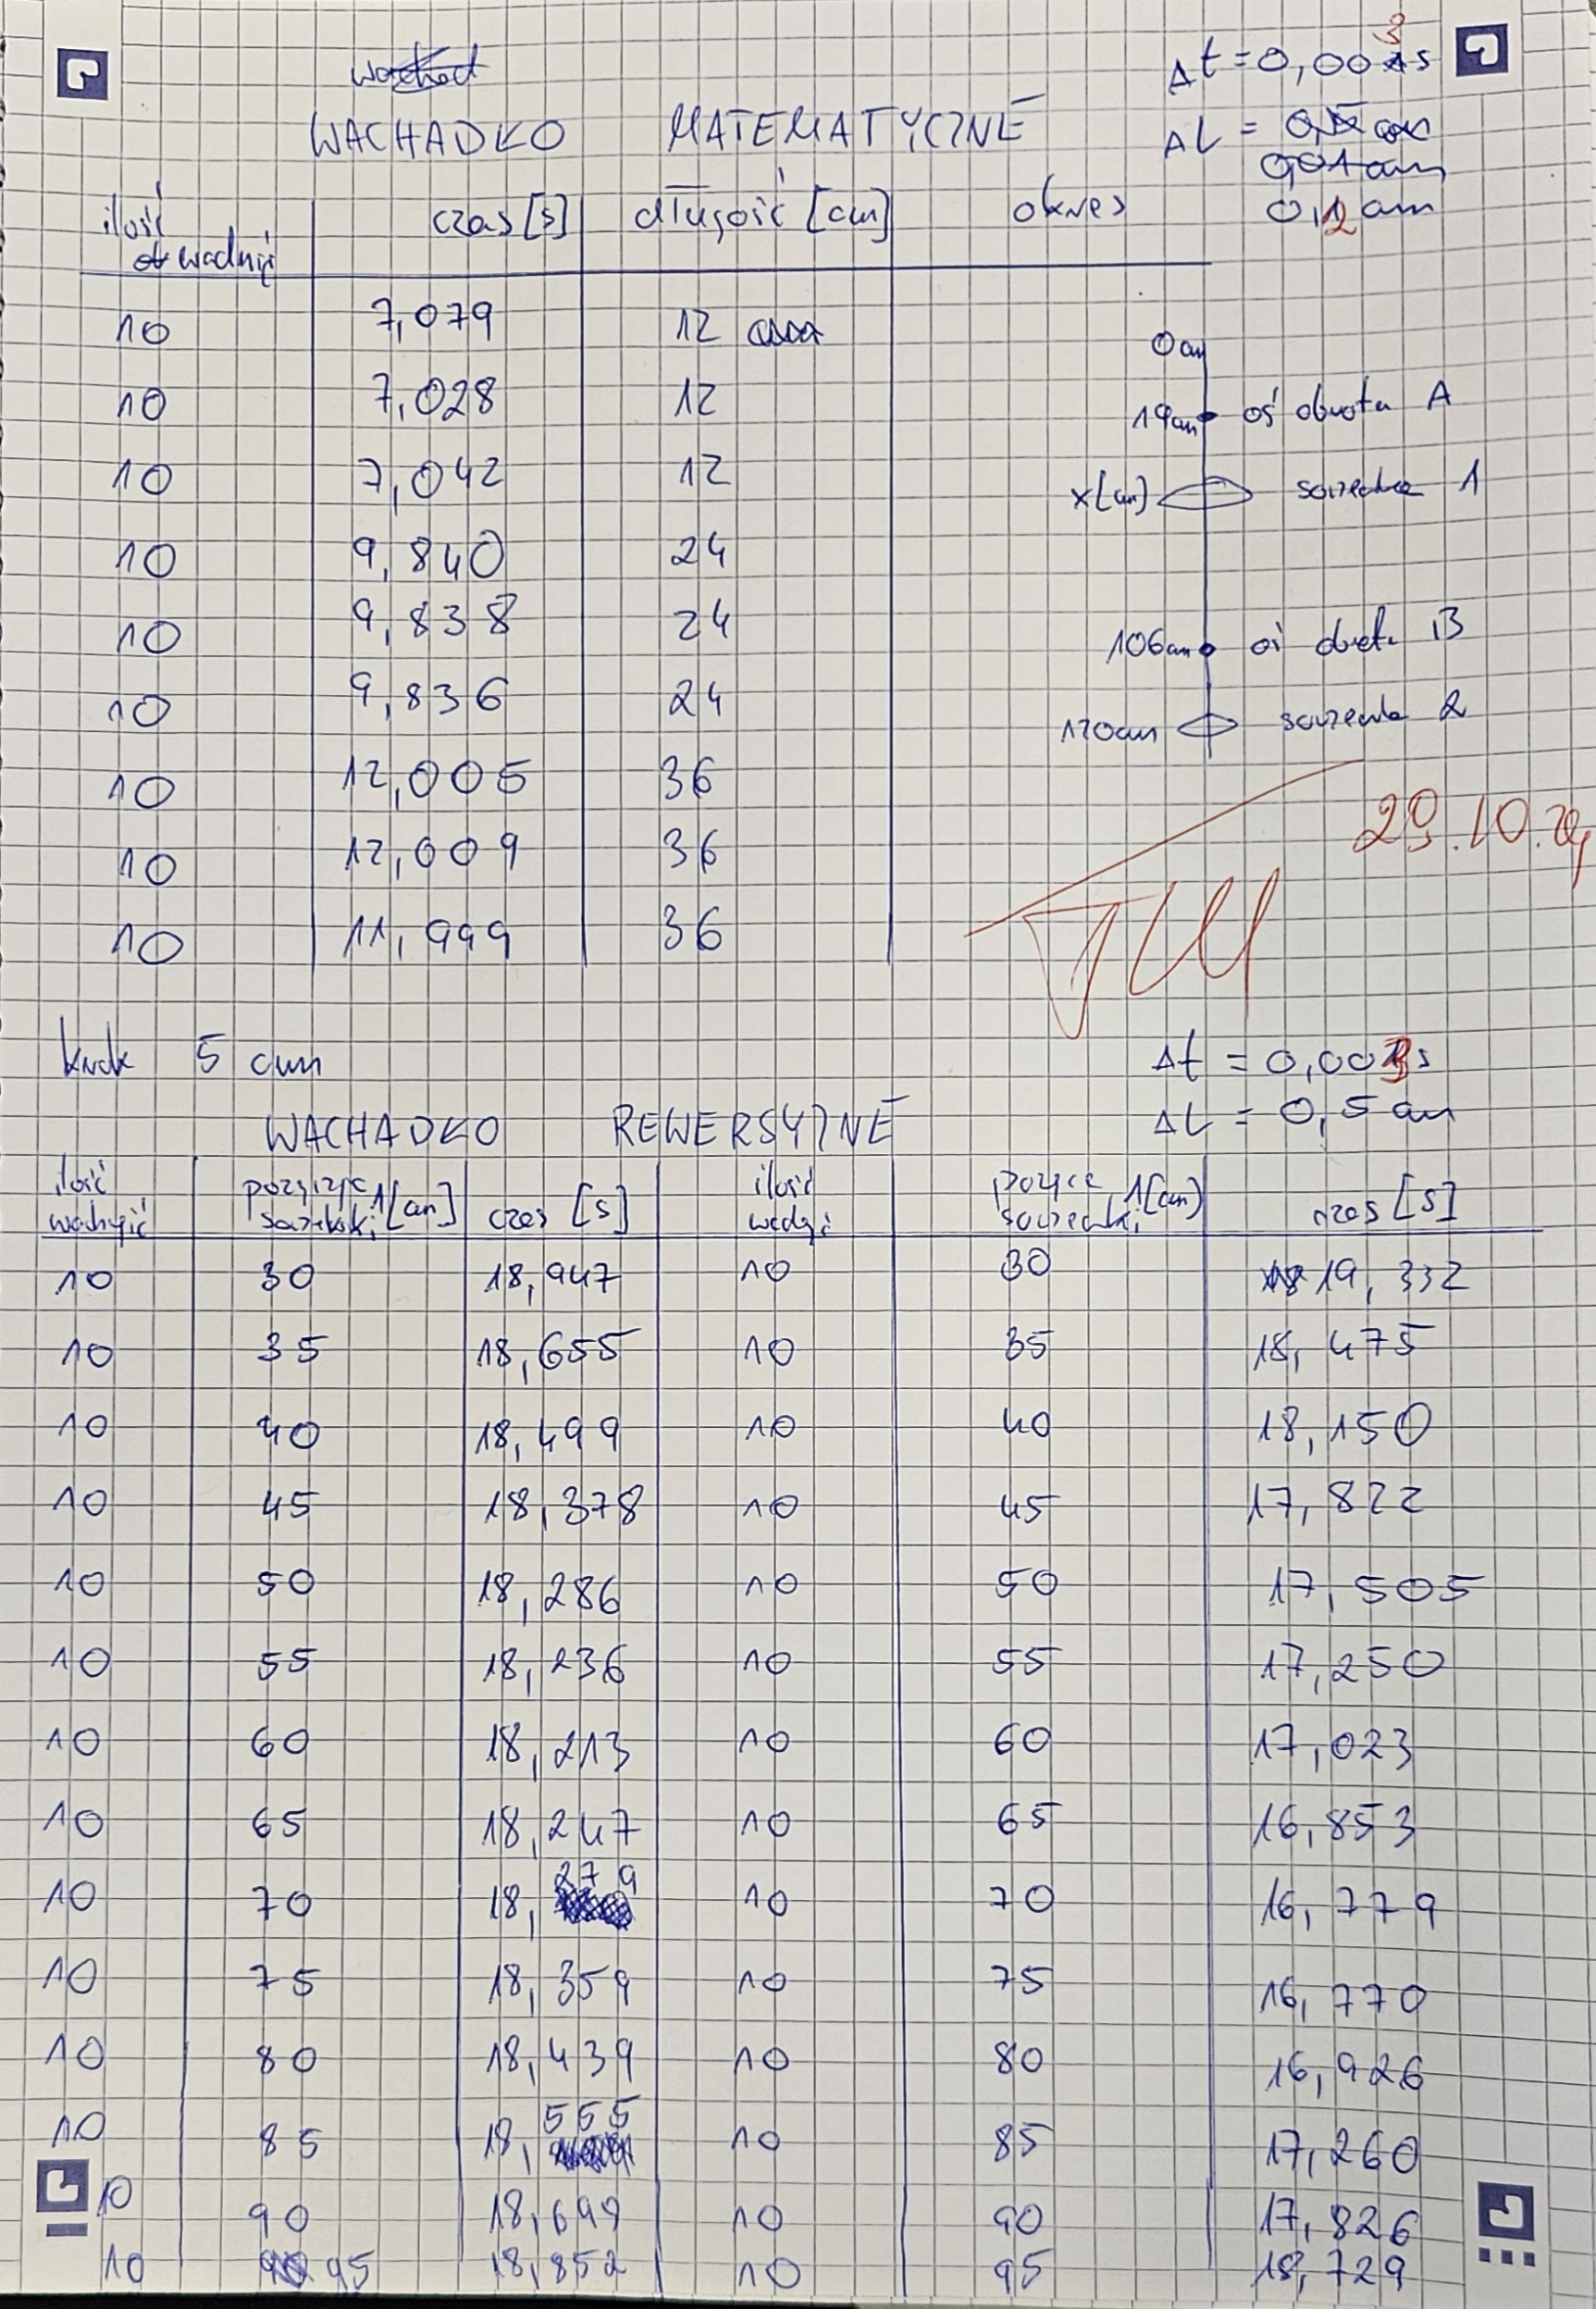
\includegraphics[scale=0.25]{images/pomiary.jpg}
\end{center}
% subsection Zdjecie wynikow pomiarow (end)

\pagebreak
\section{Opracowanie wyników}\label{sec:opracowanie_wynikow} % (fold)

\subsection{Wahadło rewersyjne}

\subsubsection{Pomiary}
\begin{adjustwidth}{-0.125\textwidth}{-0.125\textwidth}
	\begin{center}
		\begin{tabular}{|l|l|l|l|}
			\hline
			liczba wahnięć & dystans [cm] & czas [s] & okres [s] \\ \hline
			10             & 30           & 18.947   & 1.8947    \\ \hline
			10             & 35           & 18.655   & 1.8655    \\ \hline
			10             & 40           & 18.499   & 1.8499    \\ \hline
			10             & 45           & 18.378   & 1.8378    \\ \hline
			10             & 50           & 18.286   & 1.8286    \\ \hline
			10             & 55           & 18.236   & 1.8236    \\ \hline
			10             & 60           & 18.213   & 1.8213    \\ \hline
			10             & 65           & 18.247   & 1.8247    \\ \hline
			10             & 70           & 18.279   & 1.8279    \\ \hline
			10             & 75           & 18.359   & 1.8359    \\ \hline
			10             & 80           & 18.439   & 1.8439    \\ \hline
			10             & 85           & 18.555   & 1.8555    \\ \hline
			10             & 90           & 18.698   & 1.8698    \\ \hline
			10             & 95           & 18.852   & 1.8852    \\ \hline
		\end{tabular}
		\begin{tabular}{|l|l|l|l|}
			\hline
			liczba wahnięć & dystans [cm] & czas [s] & okres [s] \\ \hline
			10             & 30           & 19.332   & 1.9332    \\ \hline
			10             & 35           & 18.475   & 1.8475    \\ \hline
			10             & 40           & 18.15    & 1.815     \\ \hline
			10             & 45           & 17.822   & 1.7822    \\ \hline
			10             & 50           & 17.505   & 1.7505    \\ \hline
			10             & 55           & 17.25    & 1.725     \\ \hline
			10             & 60           & 17.023   & 1.7023    \\ \hline
			10             & 65           & 16.853   & 1.6853    \\ \hline
			10             & 70           & 16.779   & 1.6779    \\ \hline
			10             & 75           & 16.77    & 1.677     \\ \hline
			10             & 80           & 16.926   & 1.6926    \\ \hline
			10             & 85           & 17.26    & 1.726     \\ \hline
			10             & 90           & 17.826   & 1.7826    \\ \hline
			10             & 95           & 18.729   & 1.8729    \\ \hline
		\end{tabular}
	\end{center}
\end{adjustwidth}
Dokładność pomiaru czasu wynosi $\Delta t = \pm0,003$, a pomiaru długości $\Delta l = \pm0,5cm$.

\subsubsection{Wyznaczenie miejsca przecięcia wykresów.}
\begin{center}
	\begin{tikzpicture}
		\node (img) {
			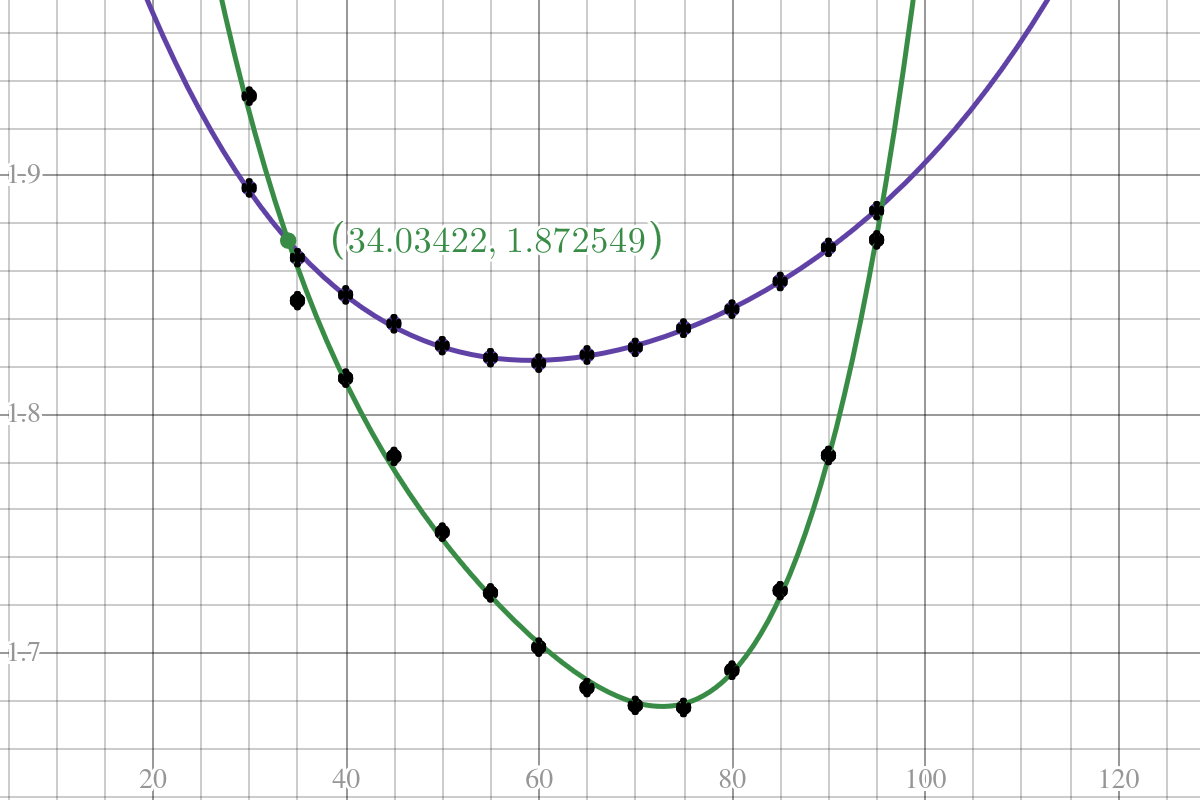
\includegraphics[scale=0.3]{images/desmos-graph.png}
		};
		\draw[->, thick] (img.south west) -- (img.south east) node[anchor=north east] {dystans [cm]};
		\draw[->, thick] (img.south west) -- (img.north west) node[anchor=north west] {okres [s]};
	\end{tikzpicture}
\end{center}
Okres dla którego $l_r = 106cm - 19cm = 87cm$ wynosi 1,8725 s.

\subsubsection{Obliczenia}
Wartość przyspieszenia ziemskiego obliczamy ze wzoru \eqref{eq:g_rew},
a błąd metodą różniczki logarytmicznej.
W tym celu przekształcamy wzór \eqref{eq:g_rew}:
\[
	g = \frac{4\pi^2l_r}{T^2_f}
\]
\[
	g = 4\pi^2 \cdot l_r \cdot\left(T^2_f\right)^{-1}
\]
\[
	g = 4\pi^2\cdot l_r \cdot T^{-2}_f
\]
\begin{equation}
	\Delta g = \left( \frac{\Delta l_r}{l_r} +2\frac{\Delta T_f}{T_f} \right)g
\end{equation}

\begin{multicols}{2}
	\[
		g = \frac{4\pi^2l_r}{T^2_f}
	\]
	\[
		g = \frac{4\pi^2 \cdot 0,87}{1,8725^2} \quad [\frac{m}{s^2}]
	\]
	\[
		g = \frac{34,311}{3,506} \quad[\frac{m}{s^2}]
	\]
	\[
		g = 9,786 \quad[\frac{m}{s^2}]
	\]

	\columnbreak

	\[
		\Delta g = \left( \frac{\Delta l_r}{l_r} +2\frac{\Delta T_f}{T_f} \right)g
	\]
	\[
		\Delta g = \left( \frac{0,002}{0,87} +2 \cdot \frac{0,003}{1,8725} \right) \cdot 9,786 \quad [\frac{m}{s^2}]
	\]
	\[
		\Delta g = \left( 0,0023 + 0,0032 \right) \cdot 9,786 \quad [\frac{m}{s^2}]
	\]
	\[
		\Delta g = 0,0538 \quad [\frac{m}{s^2}]
	\]
\end{multicols}

\subsubsection{Wynik}
\begin{equation}
	\huge  g = (9,79 \pm 0,05) \frac{m}{s^2}
\end{equation}


\subsubsection{Wnioski}
Tablicowa wartość przyśpieszenia ziemskiego mieści się w wyznaczonym zakresie.

\subsection{Wahadło matematyczne}

\subsubsection{Pomiary}
\begin{center}
	\begin{tabular}{|l|l|l|l|}
		\hline
		liczba wahnięć & czas [s] & długość [cm] & okres [s] \\ \hline
		10             & 7.079    & 12           & 0.7079    \\ \hline
		10             & 7.028    & 12           & 0.7028    \\ \hline
		10             & 7.042    & 12           & 0.7042    \\ \hline
		10             & 9.84     & 24           & 0.984     \\ \hline
		10             & 9.838    & 24           & 0.9838    \\ \hline
		10             & 9.836    & 24           & 0.9836    \\ \hline
		10             & 12.005   & 36           & 1.2005    \\ \hline
		10             & 12.009   & 36           & 1.2009    \\ \hline
		10             & 11.999   & 36           & 1.1999    \\ \hline
	\end{tabular}

\end{center}
Dokładność pomiaru czasu wynosi $\Delta t = \pm0,003$, a pomiaru długości $\Delta l = \pm0,2cm$.

\subsubsection{Wartości uśrednione i odchylenie standardowe}
\begin{center}
	\begin{tabular}{|l|l|l|l|}
		\hline
		liczba wahnięć & długość[cm] & okres\textsubscript{agv} [s] & $\sigma$okres [s] \\ \hline
		10             & 12          & 0.70                         & 0.003             \\ \hline
		10             & 24          & 0.98                         & 0.0002            \\ \hline
		10             & 36          & 1.2                          & 0.001             \\ \hline
	\end{tabular}
\end{center}

\subsubsection{Obliczenia}
Wartość przyspieszenia ziemskiego obliczamy ze wzoru \eqref{eq:g_mat},
a błąd metodą różniczki logarytmicznej.
W tym celu przekształcamy wzór \eqref{eq:g_mat}:
\[
	g = \frac{4\pi^2l}{T^2_M}
\]
\[
	g = 4\pi^2 \cdot l \cdot\left(T^2_M\right)^{-1}
\]
\[
	g = 4\pi^2\cdot l \cdot T^{-2}_M
\]
\begin{equation}
	\Delta g = \left( \frac{\Delta l}{l} +2\frac{\Delta T_M}{T_M} \right)g
\end{equation}

Przykładowo dla wahadła o długości 12cm obliczenia wyglądają następująco:
\begin{multicols}{2}
	\[
		g = \frac{4\pi^2l}{T^2_M}
	\]
	\[
		g = \frac{4\pi^2 \cdot 0,12}{0,705^2} \quad [\frac{m}{s^2}]
	\]
	\[
		g = \frac{4,7374}{0,497} \quad[\frac{m}{s^2}]
	\]
	\[
		g = 9,5315 \quad[\frac{m}{s^2}]
	\]

	\columnbreak

	\[
		\Delta g = \left( \frac{\Delta l}{l} +2\frac{\Delta T_M}{T_M} \right)g
	\]
	\[
		\Delta g = \left( \frac{0,002}{0,12} +2 \cdot \frac{0,003}{0,705} \right) \cdot 9,5315 \quad [\frac{m}{s^2}]
	\]
	\[
		\Delta g = \left( 0,0166 + 0,00852 \right) \cdot 9,5315 \quad [\frac{m}{s^2}]
	\]
	\[
		\Delta g = 0,2394 \quad [\frac{m}{s^2}]
	\]
\end{multicols}

\subsubsection{Wyniki}
\begin{center}
	\begin{tabular}{|l|l|l|l|l|l|}
		\hline
		liczba wahnięć & długość [cm] & okres\textsubscript{agv} [s] & $\sigma$ okres [s] & g [$\frac{m}{s^2}$] & $\Delta$g [$\frac{m}{s^2}$] \\ \hline
		10             & 12           & 0.70                         & 0.003              & 9.53                & 0.24                        \\ \hline
		10             & 24           & 0.98                         & 0.0002             & 9.79                & 0.14                        \\ \hline
		10             & 36           & 1.2                          & 0.001              & 9.9                 & 0.1                         \\ \hline
	\end{tabular}
\end{center}

\subsubsection{Wnioski}
Wartość tablicowa przyśpieszenia ziemskiego mieści się w przedziałach wyznaczonych dla wahadła o długościach 24 i 36 cm.
Na niedokładność wahadła o długości 12cm mógł wpłynąć fakt, że metalowa kula zawieszona na cienkiej nici nie jest idealnym wahadłem matematycznym,
jej masa nie jest skupiona w jednym punkcie, oraz działają na nią opory powietrza.


\end{document}

